\documentclass[12pt]{beamer}
\usetheme{Boadilla}

\usepackage[utf8]{inputenc}
\usepackage[english]{babel}
\usepackage{amsmath}
\usepackage{amsfonts}
\usepackage{amssymb}
\usepackage{graphicx}
\usepackage{algpseudocode}

\author{Kamal Bentahar}
\title{Investigating 3SAT}
\subtitle{(Guide presentation for 380CT Coursework 2)}
\date{\today}


\setbeamercovered{transparent}
\setbeamertemplate{navigation symbols}{}

\begin{document}
	\maketitle
	
\begin{frame}{Notation}
	Let $x_1,x_2,\ldots,x_n$ be Boolean variables, and let $\phi$ be a Boolean formula written in 3-cnf form
	\[
	\phi = c_1\land c_2\land \cdots \land c_\ell,
	\]
where each $c_m=x_i\lor x_j\lor x_k$ for some $i,j,k=1,2,...,n$.
\end{frame}

\begin{frame}{Definition of the problem}
	\begin{block}{Decisional 3SAT}
		Given a boolean expression in 3-CNF form, decide if it is satisfiable.
	\end{block}

	\begin{block}{Computational 3SAT}
		Given a boolean expression in 3-CNF form, find a satisfying assignment if satisfiable.
	\end{block}

	\begin{block}{Optimization 3SAT}
		Given a boolean expression in 3-CNF form, find an assignment that minimizes the number of non-satisfying clauses.
	\end{block}
\end{frame}

\begin{frame}
{Exhaustive search -- theory}

\begin{algorithmic}[1]\sffamily
\For{all possible variable assignments of $x_1,x_2,\ldots,x_n$}
	\If {$\phi(x_1,x_2,\ldots,x_n)$ evaluates to True}
	\State {\Return True}
	\EndIf
\EndFor
\State \Return False
\end{algorithmic}

\vfill

There are $2^n$ possible assignments, and each  evaluation of $\phi$ costs $O(\ell)$. So this algorithm costs \[O(\ell\, 2^n).\]
\end{frame}

\begin{frame}
{Exhaustive search -- empirical results}

\begin{center}
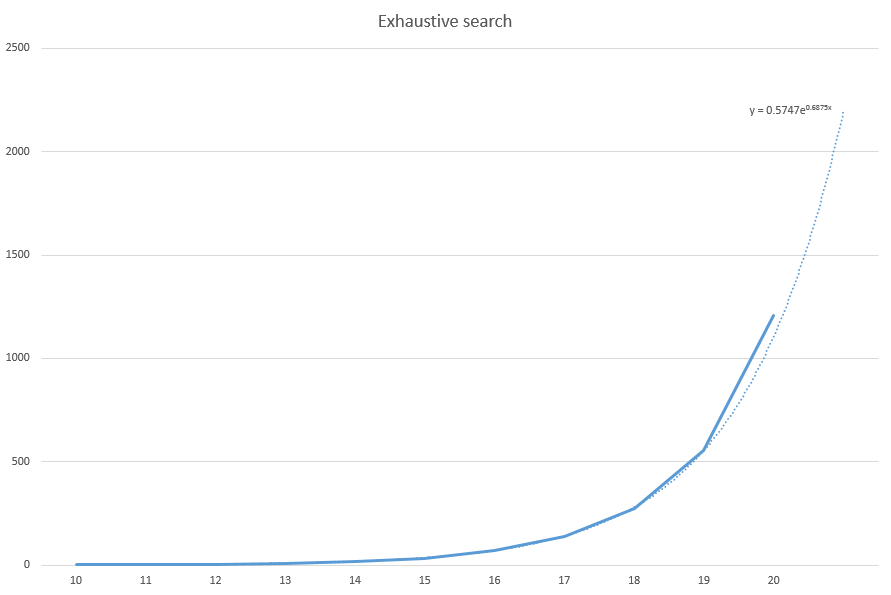
\includegraphics[width=0.7\textwidth]{img/exh2}
\end{center}

Average time in seconds for randomly generated instances with $n=\ell$ for $n=10,\ldots,20$.

Dotted line: fitted exponential curve.

\end{frame}

\end{document}